%%
%% Time-stamp: <2020-03-11 22:35:48 stefan>
%%

\documentclass[swedish,10pt,a4paper]{report}

\usepackage[utf8]{inputenc}  %% UTF8 i input

\usepackage{lmodern}         %% Latin Moderna istället för Computer Modern
\usepackage[T1]{fontenc}     %% åäö som enskilda tecken i font

\usepackage{hyperxmp}
\usepackage[unicode]{hyperref}  %% hyperlänkar mellan text och bibliografin

%% \renewcommand{\baselinestretch}{1.5}
%% \linespread{1.5}

%% smallare marginal för anteckningar
%% \usepackage[marginparwidth=30pt]{geometry}

%% \usepackage{mathptmx} %% använd Times istället för Computer Modern
%% \usepackage{mathpazo} %% använd Palatino istället för Computer Modern
\usepackage{newtxtext,newtxmath} %% annan font i math miljöer

\usepackage[english,main=swedish]{babel}          %% babel : styckenamn på svenska osv (english
                                                  %% är med tanke på korrekt funktion i citeringar)
\usepackage[strict=true,autostyle=true]{csquotes} %% csquotes - bättre citeringar i texten, beroende av babel för svenska

%% tabeller
\usepackage[flushleft]{threeparttable}                %% fotnoter inuti tabellerna
\usepackage{booktabs}                                 %% bottomrule/toprule i tabeller
\usepackage{tabu}                                     %% förbättrat layout av tabeller
\usepackage{tabularx}               %% mer användbara tabeller
\usepackage{colortbl}               %% grå bakgrund i tabeller

\usepackage{xcolor}                   %% \definecolor, den gråa bakgrunden i kodlistningarna
\definecolor{kodbakgrund}{gray}{0.95}
\definecolor{light-gray}{gray}{0.95}

\newcolumntype{s}{>{\columncolor[gray]{0.95}} p{4cm}} %% ny kolumntyp för tabeller

%% \usepackage[bottom]{footmisc} %% fotnötter i sidans nederkant
%% \usepackage{verbatim}         %% verbatim miljö
%% \usepackage{footnote}
%% \usepackage{color}

%% PDF-inkludering
\usepackage{graphicx}
%% \usepackage{pst-pdf}

% \usepackage[fleqn]{mathtools}
% \usepackage{pgf}
% \newcommand{\BinaryAdd}[2]{%
% {#1}_2 + {#2}_2 = \pgfmathbin{0b#1 + 0b#2}% compute binary addition
% \pgfmathresult_2% format output to make it clear it is base 2
% }%

\usepackage{listings} %% programkodslistningar
\lstset{basicstyle=\footnotesize,
  captionpos=b,
  backgroundcolor=\color{kodbakgrund},
  extendedchars=true,
  breaklines=true,
  literate={ö}{{\"o}}1 {å}{{\aa}}1 {Å}{{\aA}}l {ä}{{\"a}}1 {Ö}{{\"O}}1 {Ä}{{\"A}}1,
  language=Java
}

%% \usepackage[style=alphabetic,backend=biber]{biblatex}    %% biblatex behöver csquotes om babel ska användas
\usepackage[style=authoryear-ibid,backend=biber]{biblatex}   %% biblatex behöver csquotes om babel ska användas
\addbibresource[location=local]{bib.bib}
\addbibresource[location=local]{rfc.bib}
\addbibresource[location=local]{rfc_draft.bib}
\addbibresource[location=local]{pelkey.bib}
\addbibresource[location=local]{reports.bib}

% \usepackage{fancyhdr}
% \fancyhead[L]{IT119G\\Datorkommunikation}
% \fancyhead[R]{\thepage}
% \fancyfoot[L,C,R]{}
% \renewcommand{\headrulewidth}{0.2pt}
% \pagestyle{fancy}

\title{%
  Labbrapport IT119G}
\author{%
  Stefan Niskanen Skoglund\\
  IT119G\\
  19670927--5934}
\hypersetup{%
  pdftitle={%
    Labbrapport IT119G Datakommunikation
  },
  pdfauthor={%
    Stefan Niskanen Skoglund  19670927--5934
  },
  pdfsubject={%
    Labbrapport IT119G Datakommunikation
  },
  pdfkeywords={%
    Datakommunikation,
    IEEE802.3,
    IEEE802.2,
    DNS,
    IP,
    UDP,
    TCP,
    ARP,
    RARP
  }
}

\usepackage[toc,page,title]{appendix}

\begin{document}

\maketitle

\chapter{Inledning}\label{chap:inledning}

Jag kommer att presentera något om IEEE:standarderna 802.3 (standardiserad EtherNet) och LLC (Logical Link Control), ARP (Address Resolution Protocol),
IP (Internet Protocol) och DHCP (Dynamic Host Configuration Protocol.) Det finns några förutsättningar i grunden i XEROX EtherNet och DIX som även idag påverkar 802.3ae.

Avslutningen kommer att handla om DNS (Domain Name System)
och hur man kan lyssna till IP:trafik och ge exempel på orsaker till att man vill kunna göra detta.

Det sista kapitlet är en kort beskrivning av CFEngine (en
medlyssning till en hämtning via CFEngine av en fil
finns med i avlyssningskapitlet.)

\chapter{IEEE 802.3 (Ethernet)}\label{IEEE8023Ethernet}

IEEE 802.3 10base5 och 10base2 är några tidiga tekniker för anslutning
av datorer i lokala nätverk som ursprungligen utvecklades vid XEROX PARC
med tanke på deras framtida kontorsautomatiseringssystem.

Senare övertalades XEROX att istället för att se EtherNet som ett konkurrensfördel
i konkurrensen med andra leverantärer och därmed lämpligt att behålla för sig själva (vilket
är en definition av proprietära programvara och system)
att det var mer fördelaktigt för dem att låta andra leverantörer använda de här teknikerna.

XEROX bildade ett konsortium med kretstillverkaren Intel och systemleverantören
Digital Equipment Corporation där i avtalet angavs en rollfördelning mellan medlemmarna.

\section{XEROX, DIX och Robert Metcalfe }\label{sec:DIX_standard}

Ethernet utvecklades vid XEROX utvecklingscentrum i Palo-Alto\footcite{Pelkey}
som ett del i XEROX vision av hur framtidens kontorsarbetare skulle
kunna använda enpersonsdatorer, tjänster i ett nätverk inklusive de
nya laserskrivarna och kommunicera och interagera med varandra.

Kontorsarbetet ska ses som det konstruktionsarbete som en ingenjör eller
en programmerares dokumentation av sitt arbete eller den framtida
programvaruprodukten.

Enpersonsdatorer är maskiner som har tillräckligt låga driftkostnader
och är av sådan art vad beträffar handhavande så att en ingenjör
eller en sekreterare ska kunna ha ett för deras bruk reserverat exemplar.
Detta till skillnad från 1970-talets mini- och stordatorer som antingen var för
dyra eller vars skötsel var för krävande för att man skulle kunna ha dem i många exemplar.

Dock, IBM PC, Apple II och Xerox Alto var inte de första maskinerna med tillräckligt
låga kostnader för att den inte skulle kunna reserveras för en längre tid för en ingenjörs
enskilda bruk.

Bendix G-15\footcite{BendixG15brochure}, LINC (Laboratory INstrument Computer)\footcite{LINCLightsout}
och olika modeller av DEC PDP-8 räknas som de maskiner som var först att ha rätt pris och
vara så pass enkel att använda, att exempelvis en ingenjör som i sitt arbete har optimiseringsproblem att beräkna
kunde få en sådan reserverad för sitt eget bruk.

% XEROX Alto och Star (en förädlad och kommersialiserad version av Alto:maskinen som i huvudsak var prototyper och utvecklingssystem
% avsedda för intern användning) kan räknas som den första arbetsstationen i betydelsen en-användaredator med ett grafiskt
% gränssnitt, en stor katodstråleskärm, ett roterande skivminne
% och Doug Engelbarts pekdon, en mus.



Robert Metcalfe anställdes vid PARC 1972 bland annat på grund av sina erfarenheter av ARPANET
med avsikten att han skulle forska inom XEROX kontorsautomatiseringsprojekt\footcite[kap 6 sekt 7]{PelkeyChap6s7}
och ansvara för deras IMP:maskin dvs den dåtida routern mellan Arpanet och de lokala maskinerna.

Metcalfes doktorsavhandling baserades på hans arbete inom Arpanet-projektet men refuserades vid disputationen
våren 1972 med motivationen att dess matematiska innehåll var otillräckligt och att det saknas konkreta teorier
dessutom var det matematiska innehållet otillräckligt.
Norman Abramsons text\footcite{AbramsonAloha} ansåg han vara felaktig vad
beträffar modelleringen av hur människor reagerar när en förbindelse har
större och märkbara fördröjningar. Modellen i Abramsons text hade som en förutsättning att människor fortsätter
att mata in text även när svaren från värddatorn är kraftigt fördröjda.

Metcalfe frågade sin nya arbetsgivare XEROX om lov att under en period
gästforska vid Hawaiis universitet i Abramsons grupp med avsikt att slutföra avhandlingen
och fick godkänt.
Han fick ävenså bifall från Norman Abramson och gruppen till
att få komma som gästforskare.

Hans målsättning var modellering av användarnas reaktioner när förbindelser är överlastade
och formulering av matematiska teorier för detta.

Analysen tydliggjorde att orsaken till fördröjningsproblemen var de alldeles för många omsändningarna av
data när ALOHAnätet är högt utnyttjat, problemet kunde därmed identifieras som ett processkontrollproblem.
De statistiska modeller som antog att användarna inte fortsätter trycka på tangenter utan istället
så länge förbindelsen är långsam tar korta pauser, kunde visa på en möjlig problemlösning.

Den här modellen skiljer sig mot den modell som förutsätts i Poissonfördelningen
i Norman Abramsons artikel.

Idéen är att om sändaren under sändning hör att någon annan samtidigt sänder så ska man
direkt avbryta sändingen, beräkna slumpvist en längd på en väntperiod vänta den tiden ut
och därefter om ingen annan sändning har detekterats kan stationen börja sända.
och under
sluta och sedan inte ha en fast väntperiod då lär den andre också vänta ungefär samma tid ms utan
båda ska vänta ett slumpvist vald period innan ett nytt sändningsförsök
att vänta ett slumpvis antal 10-tals millisekunder innan man försöker sända. Troligtvis kommer
den andre inte vänta precis lika lång tid. Skulle det efter en sådan väntperiod under sändningen
visa sig att det fortfarande blir konflikter, ska båda stationerna vänta en ny men ungefär dubbelt så lång
väntperiod innan de försöker igen. Detta kräver att stationernas mottagningsdel fortsätter arbeta som
mottagare medan den egna stationen sänder och därmed gör det möjligt att identifiera om sändningen
tidsmässigt är i konflikt med en annan.

Detta är en central teknik i Ethernet och därmed även de olika varianterna av IEEE 802.3.

Efter att han var nöjd presenterades resultaten för Hawaiiuniversitets systemforskningsgrupp innan
han på hösten 1973 återvände till XEROX PARC där han fick ansvara för och dokumentera
hur anläggningens datorer skulle anslutas till Arpanet (IMP:maskinen hade kommit i Oktober 1973.)

Efter att förbindelsen ut var klar och igång fick han en utmaning från PARC-chefsgrupp:
\foreignquote{english}{Kan du skapa något som gör att vi kan ansluta många datorer och ett antal laserskrivare till varandra?}

XEROX patentansökan 1974\footcite[kap 6 sekt 7]{Pelkey} för Ethernet angav Robert Metcalfe, David Boggs, Butler Lampson och Chuck Thacker
som meduppfinnare. Avsikten från XEROX sida var då att Ethernet skulle vara en viktig komponent i
framtida kontorsprodukter.
Den här versionen av Ethernet var den ursprungliga versionen med 3 megabit överföringshastighet,
och som gulfärgad koaxialkabel där anslutningen görs med sk.\@vampyr-anslutning.

Metcalfe 1977--1978 frustrerad av XEROX oförmåga att bygga och sälja produkter
med den nya tekniken och att XEROX:s inställning till den var proprietär, ingen
annan skulle få använda den i sin produkt.

Metcalfe lämnade i slutet av 1978 XEROX med avsikten att i samarbete med andra
företag kommersialisera Ethernet
och därmed bli tillgängligt som tillbehör till andra datorer än de från
XEROX. Intel, Digital Equipment och XEROX bildade DIX:konsortiet som
standardiserade Ethernet som IEEE 802.3 10base5.

\foreignblockquote{english}[Robert Metcalfe]{I came to work one day at MIT and the computer had
  been stolen so I called DEC to break the news to them that this \$30,000
  computer that they'd lent me was gone. They thought this was the greatest thing that ever
  happened because it turns out I had in my possession the first computer small enough to be stolen!}

Digital Equipment hade målsättningen att till skillnad mot den äldre IMP:lösningen
kunna integrera anslutningen mot andra datornät inuti sina egna maskiner.
andra ndatornätsanslutningen inuti deras datorer.

% \includegraphics{network_diagram.tex}
%\includegraphics[height=200pt]{network_diagram_1.pdf}
%\includegraphics[width=\baselinewidth]{home_stefan_Skrivbord_IT119G_IT119G_labbrapport_network_diagram-job_176.pdf}
\begin{figure}
  \centering
  \caption{Labbnätverkets organisation}\label{network_organization}
  \fbox{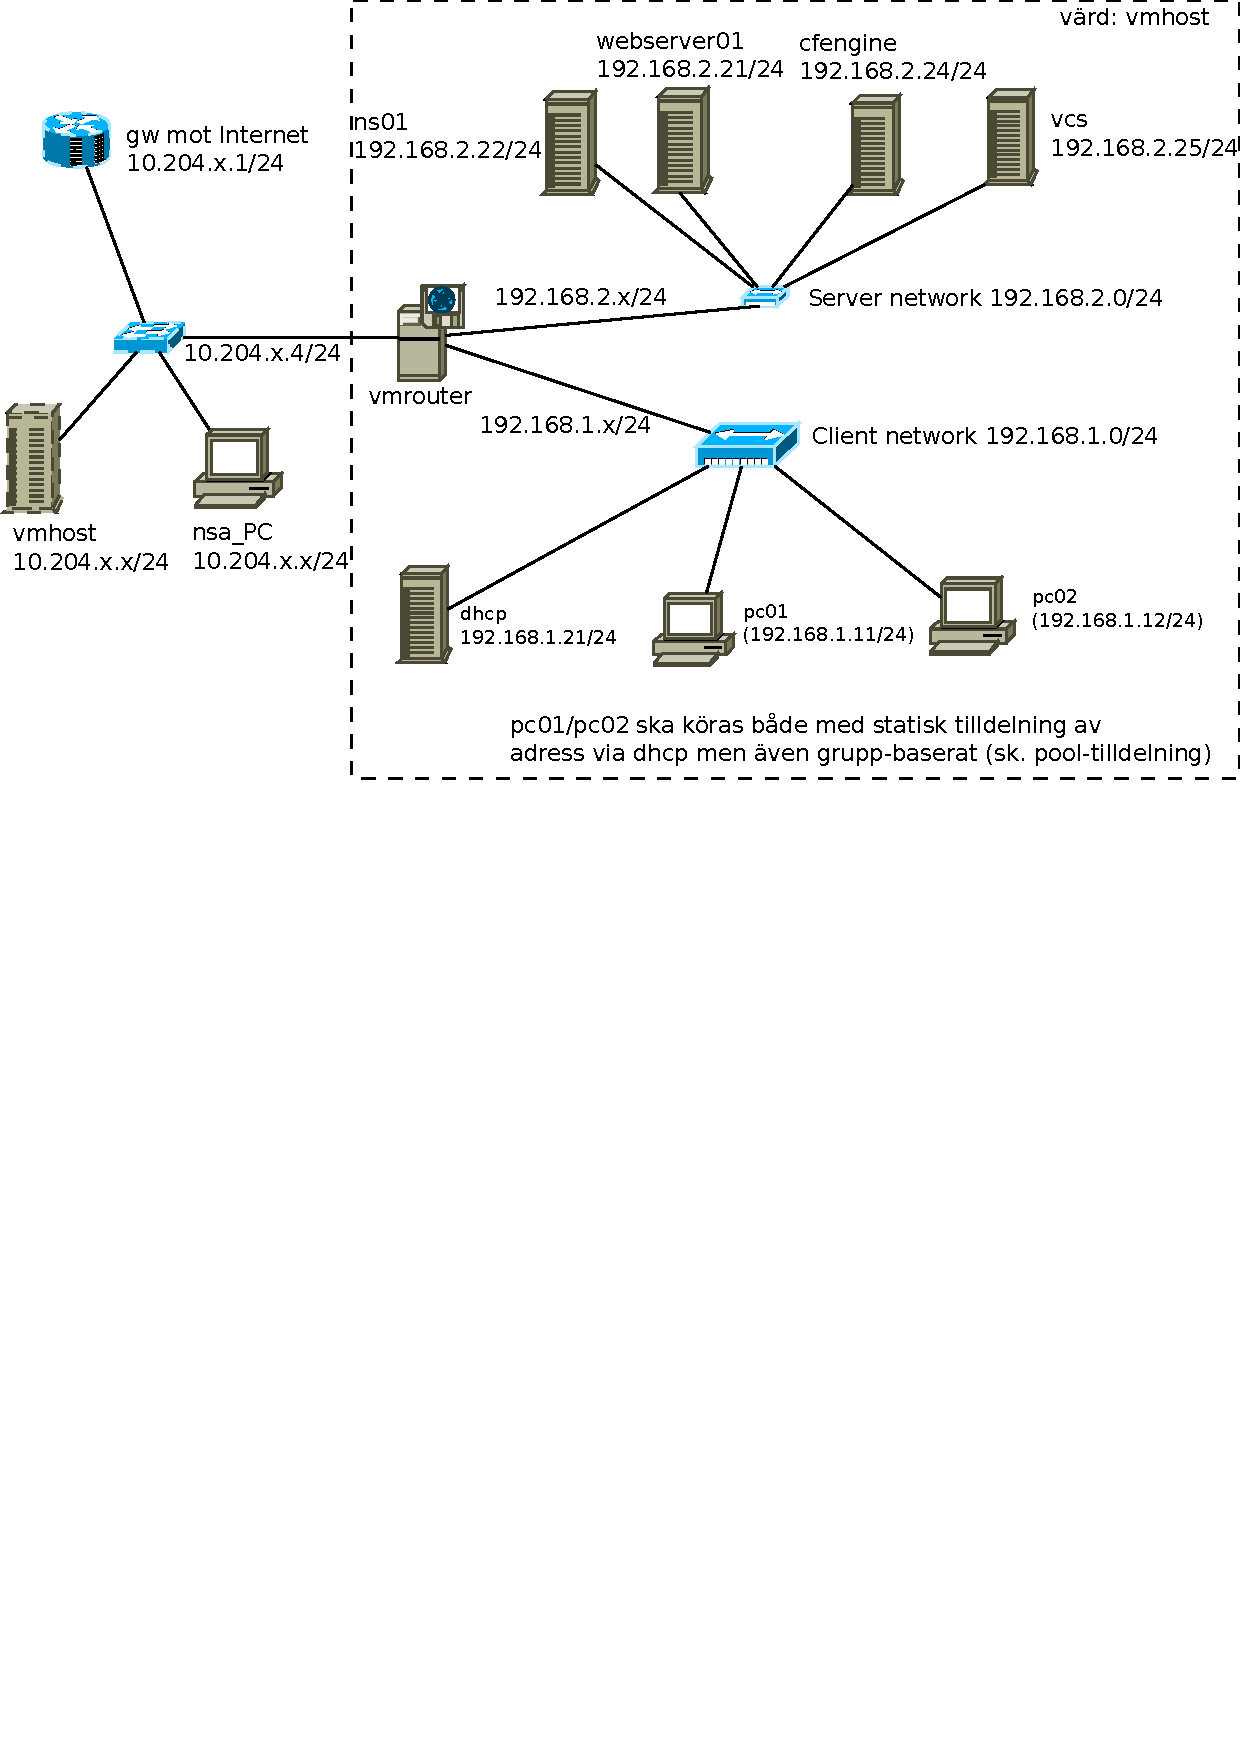
\includegraphics[width=\textwidth, clip, viewport=0 450 600 850 ]{network_diagram_export.pdf}}
\end{figure}

%% \chapter{Adressering i OSI:s länk-lager}\label{chap:adressering_i_osis_data_link_layer}

\section{Kodning i Ethernet}\label{sec:kodningiethernet}

De olika versionerna av Ethernet använder olika kodning beroende på vilken transport som
används. Jag skriver enbart om typerna Manchester och 802.3ab:s 8b/10b variant.

Fibre Channel sänder alltid i klumpar om 4 oktetter där den första oktetten anger
om de efterföljande tre är applikationsdata eller styrsignaler för förbindelsen

IEEE 802.3ab

\subsection{Manchester-kodningens fördelar}\label{subsec:manchester_pros}

Självsynkroniserande, mottagaren behöver kunna räkna fram vilka upp-
eller ner-flanker som är intressenta vilket garanteras genom den specifika
signalen (pre-amble) i ramens början som omfattar 56 stycken ettor vilket
är en stadig signal med frekvensen 20 MHz som pågår under 6 millisekunder.

\subsection{Dess nackdelar}\label{subsec:manchester_cons}

Nödvändig bandbredd i förbindelsen är fördubblas jämfört med datahastigheten.

10 Mbit IEEE 802.3 10base5 (DIX) innebär att modulationsfrekvensen i förbindelsen är 20 MHz eller 20 Mbaud.

\subsection{Fördelar i 8B/10B kodning}\label{sec:8b10bkodning}

Den mottagande photodioden lämnar en svag elektrisk signal som förstärks av
en operationsförstärkare där dess förstärkning genom återkoppling kontrolleras av en efterföljande
regulator.

\chapter{Adressöversättning i IP:baserade nätverk}\label{chap:address_translation}

Vilket protokoll används i ett nätverk där datorer vill översätta IPv4:s logiska adresser till något
som hårdvaran kan hantera? ARP = address resolution protocol.

RFC826 \footcite{rfc826} beskriver motivationen bakom och de tidiga orsakerna till ARP:s
utveckling. En viktig detalj i ARP är det faktum att det från
början utvecklades för DIX men tidigt generaliserades för att stödja
andra nätverkstekniker än DIX. DIX kom att standardiseras som IEEE 802.3 10Base5.

Generaliteten i ARP innebär att protokollet inte behövde förändras
när Ethernet bytte överföringsteknologi från en bussorienterad överföring
som i grunden fungerar som radiovågor till dagens stjärnformade nät där individuella datorer är
direkt anslutna till en för den reserverad anslutning i en sk.\ växel, anser jag.

% En växel är speciellt konstruerad för att vidarebefordra trafik från flera datorer antingen
% till dator som är ansluten i samma växel eller vidare via andra liknanden enheter till
% avsedd mottagare.

\chapter{översättning av IP-adress till de motsvarande MAC:adresserna}\label{sect:trans_ip_mac}

% \begin{table}
%   \centering
%   \caption{tabular maskinnamn \& MAC-adresser}
%   \begin{tabular}{|ss|}
%     \bottomrule
%     maskinnamn         & MAC-adress        \\
%     ESXi (vmnic0)      & 6c:0b:84:08:fa:79 \\
%     PC01 (e160)        & 00:50:56:36:16:67 \\ %% \footnote{Statisk tilldelning via gui}\\
%     webserver01 (e160) & 00:0c:29:4a:cc:d2 \\ %% \footnote{automatiskt tilldelad adress i ESXi}\\
%     \toprule
%   \end{tabular}
% \end{table}

% \begin{table}
%   \centering
%   \caption{tabularx maskinnamn \& MAC-adresser}
%   \begin{tabularx}{200pt}{|X|l|}
%     \bottomrule
%     maskinnamn         & MAC-adress       \\
%     ESXi (vmnic0)      & 6c:0b:84:08:fa:79\\
%     PC01 (e160)        & 00:50:56:36:16:67\\ %% \footnotemark[8]\\
%     webserver01 (e160) & 00:0c:29:4a:cc:d2\\ %% \footnotemark[9]\\
%     \toprule
%   \end{tabularx}
% \end{table}
%% \footnotetext[8]{Statisk tilldelning via gui}
%% \footnotetext[9]{automatiskt tilldelad adress i ESXi}

\begin{table}
  \centering
  \begin{threeparttable}{ll}
    \caption{maskinnamn med deras MAC-adresser}
    \begin{tabular}{ss} %%
      maskinnamn         & MAC-adress       \\
      ESXi (vmnic0)      & 6c:0b:84:08:fa:79\\
      PC01 (e160)        & 00:50:56:36:16:67\tnote{1}\\ %% \footnotemark[8]\\
      webserver01 (e160) & 00:0c:29:4a:cc:d2\tnote{2}\\ %% \footnotemark[9]\\
    \end{tabular}
    \begin{tablenotes}
    \item[1] {Statisk tilldelning via gui}
    \item[2] {automatiskt tilldelad adress i ESXi}
    \end{tablenotes}
  \end{threeparttable}
\end{table}

MAC-adressen för PC01 och webserver01 gäller för virtuella nätanslutningar som
definieras av ESXi och tilldelas till virtuella maskiner i den värden
men de skiljer sig från vilken OUI som de tillhör.

\chapter{ram-storlek i IEEE 802.3}\label{chap:frame_length}

Eftersom ett pakets (ram/frame) maximala överföringstid i EtherNet är standardiserad
till ett visst antal millisekunder.

\chapter{OUI = Organizationally Unique Identifier}\label{subsubsec:oui}

OUI\footcite{rfc5342} är definierat som de första 24 binära bitarna av en adress dvs första
hälften av en adress.

Det är det sätt som adresser i MAC:systemet fördelas mellan ansvariga användare
där de fritt kan välja de 24 lägre bitarna i adressen.

En datorleverantör ger sina tillverkade maskiner en individuellt MAC:adress genom
ett 24 bitar långt serienummer som konkateneras med sin OUI.\@ IANA använder
sina egna OUI exempelvis som prefix i samband med IP:s gruppsändningsprotokoll men även
som ett sätt för en protokollansvariga organisation exv en programleverantör
som vill konstruera ett proprieärt protokoll dess egen adressrymd. Utökningarna i
ppp \footcite{rfc2153} är ett exempel på ett detta.


Vad kan man säga om vem som är leverantör av en maskin om man studerar en MAC:adress i ARP:tabellen?

% \begin{tablenotes}
% \item [1] Lenovo PC
% \item [2] Hewlett-Packard växel? Anslutning i gateway:maskin för gruppen 10.204.20.0
% \item [3] Hewlett-Packard växel? Anslutning i gateway:maskin för gruppen 10.204.8.0
% \item [4] Har använt mer än en datorgrupp
% \end{tablenotes}

MAC-adresser i klassisk Ethernet som även är känt som DIX:standarden efter
de bakomliggande leverantörerna fördelar användbara adresser genom att tilldela
leverantörerna ett eller flera prefix eller adressområden som de blev ansvarig för. MAC-adressen är 48 bitar lång
och prefixet är hälften av det dvs 24 bitar. Leverantören använder
de 24 övriga bitarna för att differentiera mellan maskiner men även anslutningskort för ethernet.

Många prefix reserverades från första början för olika användningar. Ett exempel på
sådan användning är multicast i IP:nätverk där adressen 224.20.20.2 nominerar
de maskiner som är medlemmar av en viss grupp.

Varför syns det inte någon förändring i ARP-tabellen efter att
ha försökt ping:a specifik maskin bortanför utgående anslutning ?
PC01 har i ARP:tabellen lagt till VMrouter:maskinens MAC-adress.

\chapter{Trafikspårning}
\label{sec:wireshark_usage}

Vilket protokoll använder ping\footnote{se man -s 8 ping} ? ICMP:s echo:begäran (ICMP typ 8) och ICMP:s motsvarande svarspaket (ICMP typ 0.)

Eftersom trafik till andra maskiner än de fyra som är direkt åtkomliga i ``Client network'' skickas via
``VMrouter'' behövs enbart den maskinens MAC:adress i ARP:tabellen (arp funktionen i operativsystemet hanterar
next-hop:adresser.)\@10.204.20.1 är inte någon av dem.

\chapter{Dynamisk tilldelning av IP:adresser i ett nätverk}\label{chap:dynamisk_adressering}

\section{DHCP}\label{sec:dhcp_konf}

Jag flyttade ``pc01'' till  ``Server network'' sedan klagade den maskinen på ``jag är bortkopplad !''.
Dessutom fick den inte någon ny IP:adress eftersom det inte finns någon ``DHCP'' tjänst i det nätet.

Däremot sänds det på det nätet ut ett antal ``DHCP Discover''.

Normalt sett skickas ``broadcast'':paket (mottagaradress 255.255.255.255 med avsändare 0.0.0.0) till port 67 från port 68 med UDP från
den klient som vill ha en ny adress (``DHCP Request''). Dhcp:kontrollanten svarar med ett ``DHCP ACK'' från sin
egen IPv4:adress till klientens MAC-adress med klientens korrekta IPv4:adress och andra optioner som exempelvis
korrekt DNS:maskin och DNS:domännamn i samma paket.

\chapter{loggar}

``/var/lib/dhcp/dhcpd.leases'' innehåller uppgifter om vilka klienter som har fått
automatisk tilldelade adresser via ``range'':uppgiften. Om maskinen inte syns i leases och
har en statiskt tilldelad adress så är det fullt normalt - dpcpd.leases har inte
uppgifter om maskiner vars adresser är statiskt tilldelade
som exempelvis för pc01:

% \lstset{basicstyle=\footnotesize,
% captionpos=b,
% backgroundcolor=\color{kodbakgrund},
% extendedchars=true,
% breaklines=true,
% literate={ö}{{\"o}}1 {å}{{\aa}}1 {Å}{{\aA}}l {ä}{{\"a}}1 {Ö}{{\"O}}1 {Ä}{{\"A}}1
% }
%   \begin{lstlisting}[caption={/etc/dhcp/dhcpd.conf}]
%     host  pc01 {
%     hardware ethernet 00:50:56:36:16:67;
%     fixed-address 192.168.1.11;
%   }
%   \end{lstlisting}

%   \begin{lstlisting}[caption={/var/lib/dhcp/dhcpd.leases}]
%     lease 192.168.1.11 {
%     starts 5 2019/03/29 11:25:55;
%     ends 5 2019/03/29 11:35:55;
%     cltt 5 2019/03/29 11:25:55;
%     binding state active;
%     next binding state free;
%     rewind binding state free;
%     hardware ethernet 00:50:56:36:16:67;
%     client-hostname "pc01";
%   }
%   \end{lstlisting}

\chapter{broadcastdomäner}
\label{sec:broadcastdomains}

VMrouter borde vara ansluten till tre st (det lokala arbetsgruppsnätet, Server network och Client network.)

\chapter{Adressökning i Internet}\label{chap:adress_i_internet}



\chapter{DNS:konfiguration}
\label{sec:dns_konf}

% \begin{lstlisting}[caption={Några frågor, dig +search www}]
%   ; <<>> DiG 9.9.4-RedHat-9.9.4-73.el7_6 <<>> +search www
%   ;; global options: +cmd
%   ;; Got answer:
%   ;; ->>HEADER<<- opcode: QUERY, status: NOERROR, id: 63149
%   ;; flags: qr aa rd ra; QUERY: 1, ANSWER: 2, AUTHORITY: 1, ADDITIONAL: 2

%   ;; OPT PSEUDOSECTION:
%   ; EDNS: version: 0, flags:; udp: 4096
%   ;; QUESTION SECTION:
%   ;www.b18steni.it119g.nsa.his.se.	IN	A

%   ;; ANSWER SECTION:
%   www.b18steni.it119g.nsa.his.se.	10 IN	CNAME	webserver01.b18steni.it119g.nsa.his.se.
%   webserver01.b18steni.it119g.nsa.his.se.	10 IN A	192.168.2.21

%   ;; AUTHORITY SECTION:
%   b18steni.it119g.nsa.his.se. 10	IN	NS	ns01.b18steni.it119g.nsa.his.se.

%   ;; ADDITIONAL SECTION:
%   ns01.b18steni.it119g.nsa.his.se. 10 IN	A	192.168.2.22

%   ;; Query time: 0 msec
%   ;; SERVER: 192.168.2.22#53(192.168.2.22)
%   ;; WHEN: fre mar 29 13:32:30 CET 2019
%   ;; MSG SIZE  rcvd: 136
% \end{lstlisting}

% \begin{lstlisting}[caption={Några frågor, dig -t NS b18steni.it119g.nsa.his.se.}]
%   ; <<>> DiG 9.9.4-RedHat-9.9.4-73.el7_6 <<>> -t NS b18steni.it119g.nsa.his.se.
%   ;; global options: +cmd
%   ;; Got answer:
%   ;; ->>HEADER<<- opcode: QUERY, status: NOERROR, id: 20764
%   ;; flags: qr aa rd ra; QUERY: 1, ANSWER: 1, AUTHORITY: 0, ADDITIONAL: 2

%   ;; OPT PSEUDOSECTION:
%   ; EDNS: version: 0, flags:; udp: 4096
%   ;; QUESTION SECTION:
%   ;b18steni.it119g.nsa.his.se.	IN	NS

%   ;; ANSWER SECTION:
%   b18steni.it119g.nsa.his.se. 10	IN	NS	ns01.b18steni.it119g.nsa.his.se.

%   ;; ADDITIONAL SECTION:
%   ns01.b18steni.it119g.nsa.his.se. 10 IN	A	192.168.2.22

%   ;; Query time: 0 msec
%   ;; SERVER: 192.168.2.22#53(192.168.2.22)
%   ;; WHEN: fre mar 29 13:34:03 CET 2019
%   ;; MSG SIZE  rcvd: 90
% \end{lstlisting}

% \begin{lstlisting}[caption={Några frågor, dig -t A  ns01.b18steni.it119g.nsa.his.se.}]
%   ;; global options: +cmd
%   ;; Got answer:
%   ;; ->>HEADER<<- opcode: QUERY, status: NOERROR, id: 38195
%   ;; flags: qr aa rd ra; QUERY: 1, ANSWER: 1, AUTHORITY: 1, ADDITIONAL: 1

%   ;; OPT PSEUDOSECTION:
%   ; EDNS: version: 0, flags:; udp: 4096
%   ;; QUESTION SECTION:
%   ;ns01.b18steni.it119g.nsa.his.se. IN	A

%   ;; ANSWER SECTION:
%   ns01.b18steni.it119g.nsa.his.se. 10 IN	A	192.168.2.22

%   ;; AUTHORITY SECTION:
%   b18steni.it119g.nsa.his.se. 10	IN	NS	ns01.b18steni.it119g.nsa.his.se.

%   ;; Query time: 0 msec
%   ;; SERVER: 192.168.2.22#53(192.168.2.22)
%   ;; WHEN: fre mar 29 13:35:29 CET 2019
%   ;; MSG SIZE  rcvd: 90
% \end{lstlisting}

% \begin{lstlisting}[caption={Några frågor, dig -t SOA @ns1.google.com. google.com.}]
%   ;; Got answer:
%   ;; ->>HEADER<<- opcode: QUERY, status: NOERROR, id: 24539
%   ;; flags: qr aa rd; QUERY: 1, ANSWER: 1, AUTHORITY: 4, ADDITIONAL: 9
%   ;; WARNING: recursion requested but not available

%   ;; OPT PSEUDOSECTION:
%   ; EDNS: version: 0, flags:; udp: 512
%   ;; QUESTION SECTION:
%   ;google.com.			IN	SOA

%   ;; ANSWER SECTION:
%   google.com.		60	IN	SOA	ns1.google.com. dns-admin.google.com. 240952484 900 900 1800 60

%   ;; AUTHORITY SECTION:
%   google.com.		345600	IN	NS	ns2.google.com.
%   google.com.		345600	IN	NS	ns4.google.com.
%   google.com.		345600	IN	NS	ns1.google.com.
%   google.com.		345600	IN	NS	ns3.google.com.

%   ;; ADDITIONAL SECTION:
%   ns2.google.com.		345600	IN	A	216.239.34.10
%   ns2.google.com.		345600	IN	AAAA	2001:4860:4802:34::a
%   ns4.google.com.		345600	IN	A	216.239.38.10
%   ns4.google.com.		345600	IN	AAAA	2001:4860:4802:38::a
%   ns1.google.com.		345600	IN	A	216.239.32.10
%   ns1.google.com.		345600	IN	AAAA	2001:4860:4802:32::a
%   ns3.google.com.		345600	IN	A	216.239.36.10
%   ns3.google.com.		345600	IN	AAAA	2001:4860:4802:36::a

%   ;; Query time: 25 msec
%   ;; SERVER: 216.239.32.10#53(216.239.32.10)
%   ;; WHEN: fre mar 29 13:37:10 CET 2019
%   ;; MSG SIZE  rcvd: 333
% \end{lstlisting}

% \begin{lstlisting}[caption={Några frågor, 'dig -t A www' med eller utan '+search'}]
%   dig +search www

%   ; <<>> DiG 9.10.3-P4-Ubuntu <<>> +search www
%   ;; global options: +cmd
%   ;; Got answer:
%   ;; ->>HEADER<<- opcode: QUERY, status: NOERROR, id: 61521
%   ;; flags: qr aa rd ra; QUERY: 1, ANSWER: 2, AUTHORITY: 1, ADDITIONAL: 2

%   ;; OPT PSEUDOSECTION:
%   ; EDNS: version: 0, flags:; udp: 4096
%   ;; QUESTION SECTION:
%   ;www.b18steni.it119g.nsa.his.se.	IN	A

%   ;; ANSWER SECTION:
%   www.b18steni.it119g.nsa.his.se.	10 IN	CNAME	webserver01.b18steni.it119g.nsa.his.se.
%   webserver01.b18steni.it119g.nsa.his.se.	10 IN A	192.168.2.21

%   ;; AUTHORITY SECTION:
%   b18steni.it119g.nsa.his.se. 10	IN	NS	ns01.b18steni.it119g.nsa.his.se.

%   ;; ADDITIONAL SECTION:
%   ns01.b18steni.it119g.nsa.his.se. 10 IN	A	192.168.2.22

%   ;; Query time: 0 msec
%   ;; SERVER: 192.168.2.22#53(192.168.2.22)
%   ;; WHEN: Fri Mar 29 13:42:24 CET 2019
%   ;; MSG SIZE  rcvd: 136

%   dig www

%   ; <<>> DiG 9.10.3-P4-Ubuntu <<>> www
%   ;; global options: +cmd
%   ;; Got answer:
%   ;; ->>HEADER<<- opcode: QUERY, status: NXDOMAIN, id: 44523
%   ;; flags: qr rd ra ad; QUERY: 1, ANSWER: 0, AUTHORITY: 1, ADDITIONAL: 1

%   ;; OPT PSEUDOSECTION:
%   ; EDNS: version: 0, flags:; udp: 4096
%   ;; QUESTION SECTION:
%   ;www.				IN	A

%   ;; AUTHORITY SECTION:
%   .			10692	IN	SOA	a.root-servers.net. nstld.verisign-grs.com. 2019032900 1800 900 604800 86400

%   ;; Query time: 2 msec
%   ;; SERVER: 192.168.2.22#53(192.168.2.22)
%   ;; WHEN: Fri Mar 29 13:42:33 CET 2019
%   ;; MSG SIZE  rcvd: 107
% \end{lstlisting}

\chapter{Betydelsen av punkt eller inte i frågor med dig}

Dig:programmet kan använda den sökdomän i DNS som maskinerna är konfigurerade för, ``b18steni.it119g.nsa.his.se'' i mitt fall och ``xxxx.it119g.nsa.his.se''
för övriga klasskamrater.
Dock kräver ``dig'' att flaggan ``+search'' specificeras då eller att användaren självt specificerar domännamnet.

De här frågorna är ekvivalenta:
\begin{verbatim}
dig www.
dig www
\end{verbatim}
och dessa:
\begin{verbatim}
dig www.b18steni.it119g.nsa.his.se.
dig +search www
\end{verbatim}

\chapter{DNS:konfiguration}\label{sec:dns_config}

\chapter{WEB:tjänst}\label{sec:httpd_config}

DNS i ns01 får frågan:
Jag vill få en A:uppgift för maskinen ``webserver01.b18steni.it119g.nsa.his.se''.
Har du någrar data om detta ?
BIND:programmet svarar med motsvarande A:uppgift dvs vad ``webserver01.b18steni.it119g.nsa.his.se''
heter och vilken IP:adress den har.

---
; <<>> DiG 9.10.3-P4-Ubuntu <<>> @192.168.2.22 webserver01.b18steni.it119g.nsa.his.se
; (1 server found)
;; global options: +cmd
;; Got answer:
;; ->>HEADER<<- opcode: QUERY, status: NOERROR, id: 9893
;; flags: qr aa rd; QUERY: 1, ANSWER: 1, AUTHORITY: 1, ADDITIONAL: 2
;; WARNING: recursion requested but not available

;; OPT PSEUDOSECTION:
; EDNS: version: 0, flags:; udp: 4096
;; QUESTION SECTION:
;webserver01.b18steni.it119g.nsa.his.se.	IN A

;; ANSWER SECTION:
webserver01.b18steni.it119g.nsa.his.se.	10 IN A	192.168.2.21

;; AUTHORITY SECTION:
b18steni.it119g.nsa.his.se. 10	IN	NS	ns01.b18steni.it119g.nsa.his.se.

;; ADDITIONAL SECTION:
ns01.b18steni.it119g.nsa.his.se. 10 IN	A	192.168.2.22

;; Query time: 0 msec
;; SERVER: 192.168.2.22\#53(192.168.2.22)
;; WHEN: Sun Apr 14 17:02:20 CEST 2019
;; MSG SIZE  rcvd: 118
---
Det protokoll från applikationsnivån som används är DNS (eller domain.)
Transportprotokollet för sådana här frågor är vanligtvis UDP med det
undantaget att vissa frågor pga svaren blir för stora för ett UDP:paket
sänds med TCP. Min DNS:tjänst i ns01 dvs 192.168.2.22.
Avsändningsporten är 53683 och mottagande 53 (klienten.)
Från klienten ser det ut som att svaret kommer från port 53 destinerat
till 53683.


\chapter{Uppgifter --- statisk IP:adressering}\label{sec:statisk_ip_adressering}

\begin{table}
  \centering
  \caption{maskinnamn, MAC-adresser och leverantör}
  \begin{tabular}{|sss|}
    \bottomrule
    maskinnamn         & MAC-adress        & Ansvarig leverantör\\
    ESXi (vmnic0)      & 6c:0b:84:08:fa:79 & Universal Global Scientific Industrial Co.,Ltd.\\
    PC01 (e160)        & 00:50:56:36:16:67 & VMware Inc\\
    webserver01 (e160) & 00:0c:29:4a:cc:d2 & VMware Inc\\
    dhcp01 (e160)      & 00:0c:29:9e:43:6a & VMware Inc\\
    10.204.20.1        & bc:ea:fa:11:94:33 & Hewlett-Packard\\
    10.204.8.1         & bc:ea:fa:11:94:47 & Hewlett-Packard\\
    \toprule
  \end{tabular}
\end{table}


\chapter{TCP-anslutningsfaser för en HTTP:överföring }\label{sec:tcp_phases_http}

TCP definieras som en strömbaserad tillförlitlig förbindelse där strömbaserad ska ses som
att förbindelsen ses som ett flöde utan några för applikationen direkt synliga gränser.

TCP är tillförlig i betydelsen att avsändare och mottagare ska meddelas om rapport det blir
ett avbrott i förbindelsen som medför att det hos mottagaren saknas data.
Data som leveraras till mottagande program får ävenså inte vara förvanskat och alla data ska överlämnas
i samma ordning som när det överlämnades av avsändande program till sin maskins TCP:modul.

TCP:modul ska ses som den del av operativsystem eller det användareprogram som implementerar TCP (och
underliggande moduler exv IP och ARP.) DECnet är ett exempel där användaren har installerat ett
separat program för att implementera TCP ovanför en otillförlitlig transport via IP, DECnet eller X25.

Tre-stegs handskakning
\begin{verbatim}
--
SYN
SYN+ACK
ACK
--
\end{verbatim}

\chapter{CFEngine}\label{sec:cfengine}

I arbetet har jag använt administrationsverktyget CFEngine Enterprise
för systemadministration och git som ett sätt att versionssäkra
CFEngine:s regeluppsättning.

Regeluppsättningen är en uppsättning av åtagande som ska
alltid ska hållas på för just det åtagandet aktuella system.

Åtaganden som används är:
\begin{itemize}
\item \texttt{BIND}:s egen konfiguration
\item Innehållet i \texttt{DNS}:zonerna
\item \texttt{ISC-DHCP}:kontrollants konfiguration inklusive adressuppgifterna för \texttt{pc01} och \texttt{pc02}
\item Att datakom:användaren är definierad med korrekt lösenord på \texttt{ns01}, \texttt{webserver01} och \texttt{dhcp01}
\item Att \texttt{/var/www/html/mytextfile.txt} är tillgängligt via \texttt{http} från \texttt{webserver01}
\item Att Ubuntu:s \texttt{open-vm-tools} är installerat och aktivt (\texttt{ns01}, \texttt{webserver01} och \texttt{dhcp01})
\item Att CentOS:s \texttt{open-vm-tools} är installerat och aktivt (\texttt{cfengine} och \texttt{vcs})
\end{itemize}

En git:tjänst används som revisionskontrollerad källa för de åtagande i regelsamlingen som anslutna maskiner är
förpliktade att infria och hålla.

Ansvariga administratörer beskriver ett åtagande med ett regelbaserat språk i normala
textfiler. Dessa filer med sina ändringar, registreras i det git:förråd som CFengine:s kontrollant
(även detta räknas som ett åtagande från kontrollanten) förväntas distribuera regler från.

Efter en förändring i git:förrådet hämtar kontrollanten hela den ändrade regeluppsättningen, provkör den (i huvudsak
en kontroll av syntaxen) och om kontrollen blev godkänd kommer den nya
regeluppsättningen att ersätta den som dess förinnan lämnades ut.

Maskiner som är förpliktade att följa regelsamlingen begär med ett
fast intervall ut aktuell version av reglerna från kontrollanten.

% Hämtande maskiner kontrollerar att kontrollanten alltid har samma identitet liksom
% att kontrollanten kontrollerar att hämtande maskiner har samma identitet.

% Dessutom används verktyget för att aktivera uppgraderingar av programvaran
% förutom för pc01/pc02 på de virtuella maskinerna ns01,webserver01 och dhcp01.
% Därav de extra två maskinerna cfengine och vcs \ref{network_organization} i ``server network''.
% VCS:maskinen är värd för git som används av cfengine för att sina data.
% Samma git:installation används även i rapportskrivningen.

\appendix

\addappheadtotoc

\section{DNS Konfigurationsfiler}\label{appendix:dns_conf_files}

I systemet modifierade filer inklusive DNS zonuppgifter.

Egentligen konfiguration av bind\footnote{se ``man -s 8 bind''} självt
eftersom formatet för filer som beskriver uppgifter för en zon är separat
från det format som bind:programmet använder för sin egna inställningar.

\begin{lstlisting}[caption={/etc/bind/named.conf}]
//
// avsedd för ns01.b18steni.it119g.nsa.his.se
//
// cfe-regler från 192.168.2.24
// senast uppdatering av policy:
//

include "/etc/bind/named.conf.options";
include "/etc/bind/named.conf.local";
\end{lstlisting}

\begin{lstlisting}[caption={/etc/bind/named.conf.local}]
//
// avsedd för ns01.b18steni.it119g.nsa.his.se
//
// cfe-regler från 192.168.2.24
// senast uppdatering av policy:
//

zone "b18steni.it119g.nsa.his.se" {
    type master;
    file "/etc/bind/zones/db.b18steni";
};

zone "168.192.in-addr.arpa" {
    type master;
    file "/etc/bind/zones/db.b18steni_192_rev";
};
\end{lstlisting}

\begin{lstlisting}[caption={/etc/bind/named.conf.options}]
//
// avsedd för ns01.b18steni.it119g.nsa.his.se
//
// cfe-regler från 192.168.2.24
// senast uppdatering av policy:
//

acl my_computers { 192.168.0.0/16; 10.204.12.0/24; 10.204.20.0/24; };

options {
    directory "/var/cache/bind";
    dnssec-validation auto;

    forwarders {
      10.0.252.201; // använder labbets DNS:maskiner för
      10.0.252.202; // externa frågor
    };

    listen-on-v6 { any; };
    auth-nxdomain no;    \# conform to RFC1035

    allow-recursion { my_computers; }; // neka att jobba åt andra
    allow-query { any; };              // men andra kan ställa frågor
};
\end{lstlisting}

\section{DNS zoner}\label{appendix:dns_zones}

\begin{lstlisting}[language=sh,caption={/etc/bind/zones/db.b18steni.it119g.nsa.his.se}]
# root-domain
TTL 2000
@ IN SOA ns01.b18steni.it119g.nsa.his.se. stefan.b18steni.it119g.nsa.his.se.
               (2019050218
                14400
                3600
                1209600
                600)
\end{lstlisting}

\begin{lstlisting}[language=sh,caption={/etc/bind/zones/db.1.168.192.in-addr.arpa}]
# reverse mapp ip-adresserna 192.168.1.x -> maskin-namn
$TTL 2000
\end{lstlisting}

\begin{lstlisting}[caption={/etc/bind/zones/db.2.168.192.in-addr.arpa}]
# reverse mapp ip-adresserna 192.168.2.x -> maskin-namn
$TTL 2000
\end{lstlisting}

% \texttt{db.b18steni.it119g.nsa.his.se} och motsvarande baklängesmapp\@
% \texttt{ db.192.168.2/db.192.168.1} för trädet \texttt{2.168.192.in-addr.arpa}
% och \texttt{1.168.192.in-addr.arpa}.

\section{isc dhcp kontrollantens konfiguration}\label{appendix:isc_dhcpd_config}
\subsection{poolbaserad allokering av adresser}\label{appendix:isc_dhcpd_address_pools}

\begin{lstlisting}[caption={/etc/dhcp/dhcpd.conf} (pool-baserad allokering av adresser)]
#
# avsedd för dhcp01.b18steni.it119g.nsa.his.se
#
# def.json tidsstämpel: Time-stamp: <2019-05-06 12:09:15 nsa>
# host.json tidsstämpel: Time-stamp: <2019-03-29 13:17:21 nsa>
# senast uppdatering av policy: Mon May  6 12:13:17 2019
#
# cfe-regler från 192.168.2.24
#

ddns-update-style none;

option routers 192.168.1.1;
option domain-name "b18steni.it119g.nsa.his.se";
option domain-name-servers 192.168.2.22;

option ntp-servers 194.58.203.20;
default-lease-time 600;
max-lease-time 7200;

# If this DHCP server is the official DHCP server for the local
# network, the authoritative directive should be uncommented.
authoritative;

# Use this to send dhcp log messages to a different log file (you also
# have to hack syslog.conf to complete the redirection).
log-facility local7;

#
# utan static_dhcp_mapping
#
subnet 192.168.1.0 netmask 255.255.255.0 {
  range 192.168.1.10 192.168.1.20;
  option routers 192.168.1.1;
}
\end{lstlisting}

\subsection{statisk allokering av adresser}\label{appendix:dhcp_static_allocation}

\begin{lstlisting}[caption={/etc/dhcp/dhcpd.conf} (statisk allokering av adresser)]
#
# avsedd för dhcp01.b18steni.it119g.nsa.his.se
#
# def.json tidsstämpel: Time-stamp: <2019-05-06 12:09:15 nsa>
# host.json tidsstämpel: Time-stamp: <2019-03-29 13:17:21 nsa>
# senast uppdatering av policy: Mon May  6 12:13:17 2019
#
# cfe-regler från 192.168.2.24
#

ddns-update-style none;

option routers 192.168.1.1;
option domain-name "b18steni.it119g.nsa.his.se";
option domain-name-servers 192.168.2.22;

option ntp-servers 194.58.203.20;
default-lease-time 600;
max-lease-time 7200;

# If this DHCP server is the official DHCP server for the local
# network, the authoritative directive should be uncommented.
authoritative;

# Use this to send dhcp log messages to a different log file (you also
# have to hack syslog.conf to complete the redirection).
log-facility local7;

#
# utan static_dhcp_mapping
#
subnet 192.168.1.0 netmask 255.255.255.0 {
  range 192.168.1.10 192.168.1.20;
  option routers 192.168.1.1;
}
\end{lstlisting}

\subsection{dhcpd:programmets uppskrivning av aktuella allokeringar}\label{appendix:dhcp_leases}

\begin{lstlisting}[caption={/var/lib/dhcp/dhcpd.leases}]
lease 192.168.1.11 {
  starts 5 2019/03/29 11:25:55;
  ends 5 2019/03/29 11:35:55;
  cltt 5 2019/03/29 11:25:55;
  binding state active;
  next binding state free;
  rewind binding state free;
  hardware ethernet 00:50:56:36:16:67;
  client-hostname "pc01";
}
\end{lstlisting}


\newpage
\printbibliography{}

\end{document}
